% !TEX program = xelatex
% 人工智能综合实训 II 实训报告 —— LaTeX 版本
% 编译：xelatex report.tex （建议连续编译两次以生成目录）
\documentclass[12pt,a4paper,fontset=fandol]{ctexart}   % Fandol 为 TeX Live 自带中文字体，免依赖系统字体
\usepackage[margin=2.5cm]{geometry}
\usepackage{graphicx}
\usepackage{booktabs}
\usepackage{float}
\usepackage{caption}
\usepackage{amsmath}
\usepackage{hyperref}
\hypersetup{hidelinks}

\captionsetup{font=small}
\graphicspath{{../task1_ml_wine/outputs/}{../task2_alexnet_fmnist/outputs/}}

\title{\textbf{人工智能综合实训 II 实训报告}}
\author{学号后三位\,姓名\quad（组员分工见附录）}
\date{\today}

\begin{document}
\maketitle

\begin{abstract}
\noindent 本报告完成两个机器学习项目。项目一在 UCI 白葡萄酒质量数据集上构建多分类模型，
对比支持向量机、决策树、随机森林与逻辑回归四种算法；项目二逐层手写实现经典卷积神经网络
AlexNet，在 Fashion-MNIST 图像数据集上完成十分类任务。实验表明：项目一中随机森林表现最佳，
测试集宏平均 F1 达 0.734；项目二手写 AlexNet 在测试集上达到 91.55\% 的准确率。
\par\vspace{1ex}
\noindent\textbf{关键词：}机器学习；支持向量机；随机森林；卷积神经网络；AlexNet
\end{abstract}

\tableofcontents
\newpage

\section{引言}
机器学习已广泛应用于工业质量评估、计算机视觉等领域。结构化数据的分类（如食品质量评级）
通常采用传统机器学习算法，而图像识别则依赖深度卷积神经网络。2012 年 Krizhevsky 等人提出的
AlexNet 首次在 ImageNet 大规模图像识别竞赛中以显著优势夺冠，确立了深度卷积网络在计算机视觉
中的主导地位。本报告分别以这两类任务为载体，完整实践“加载$\rightarrow$查看$\rightarrow$预处理
$\rightarrow$建模$\rightarrow$评估$\rightarrow$结论”的机器学习流程。
\textit{（此处可进一步补充研究背景、应用现状与意义。）}

\section{项目一：红酒质量分类}

\subsection{数据集与预处理}
采用 UCI 白葡萄酒质量数据集，共 4898 个样本、11 个理化特征，原始质量评分为 0--10 的整数。
为构建分类任务，将评分分箱为三类：评分 $\le 5$ 记为“差”、$=6$ 记为“中”、$\ge 7$ 记为“好”。
数据经标准化处理（仅在训练集上拟合以避免数据泄漏），并按 8:2 分层划分训练集与测试集。
针对类别不平衡，各模型统一采用类别加权（\texttt{class\_weight='balanced'}）。
图~\ref{fig:eda_dist} 与图~\ref{fig:eda_corr} 给出质量分布与特征相关性分析。

\begin{figure}[H]
  \centering
  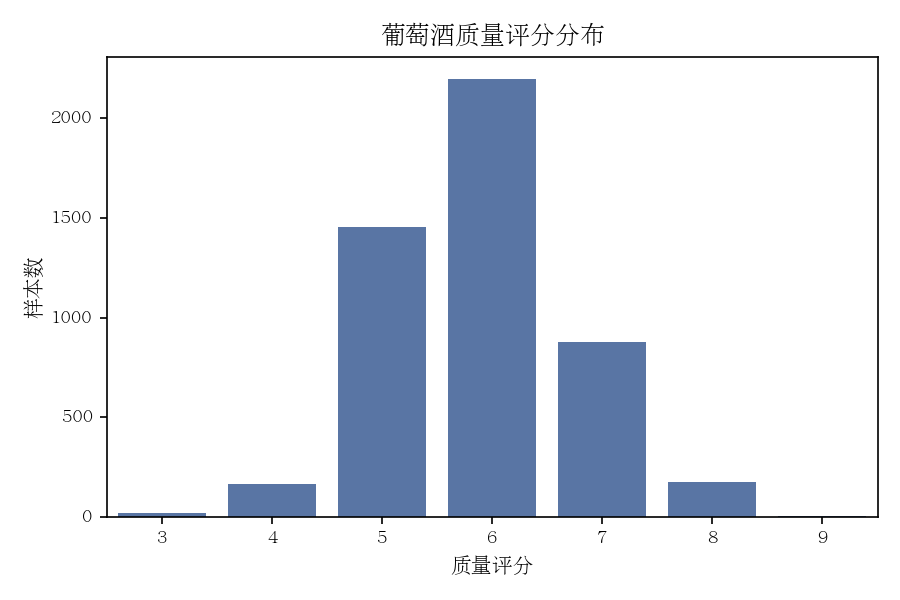
\includegraphics[width=0.6\textwidth]{eda_quality_dist.png}
  \caption{葡萄酒质量评分分布}
  \label{fig:eda_dist}
\end{figure}

\begin{figure}[H]
  \centering
  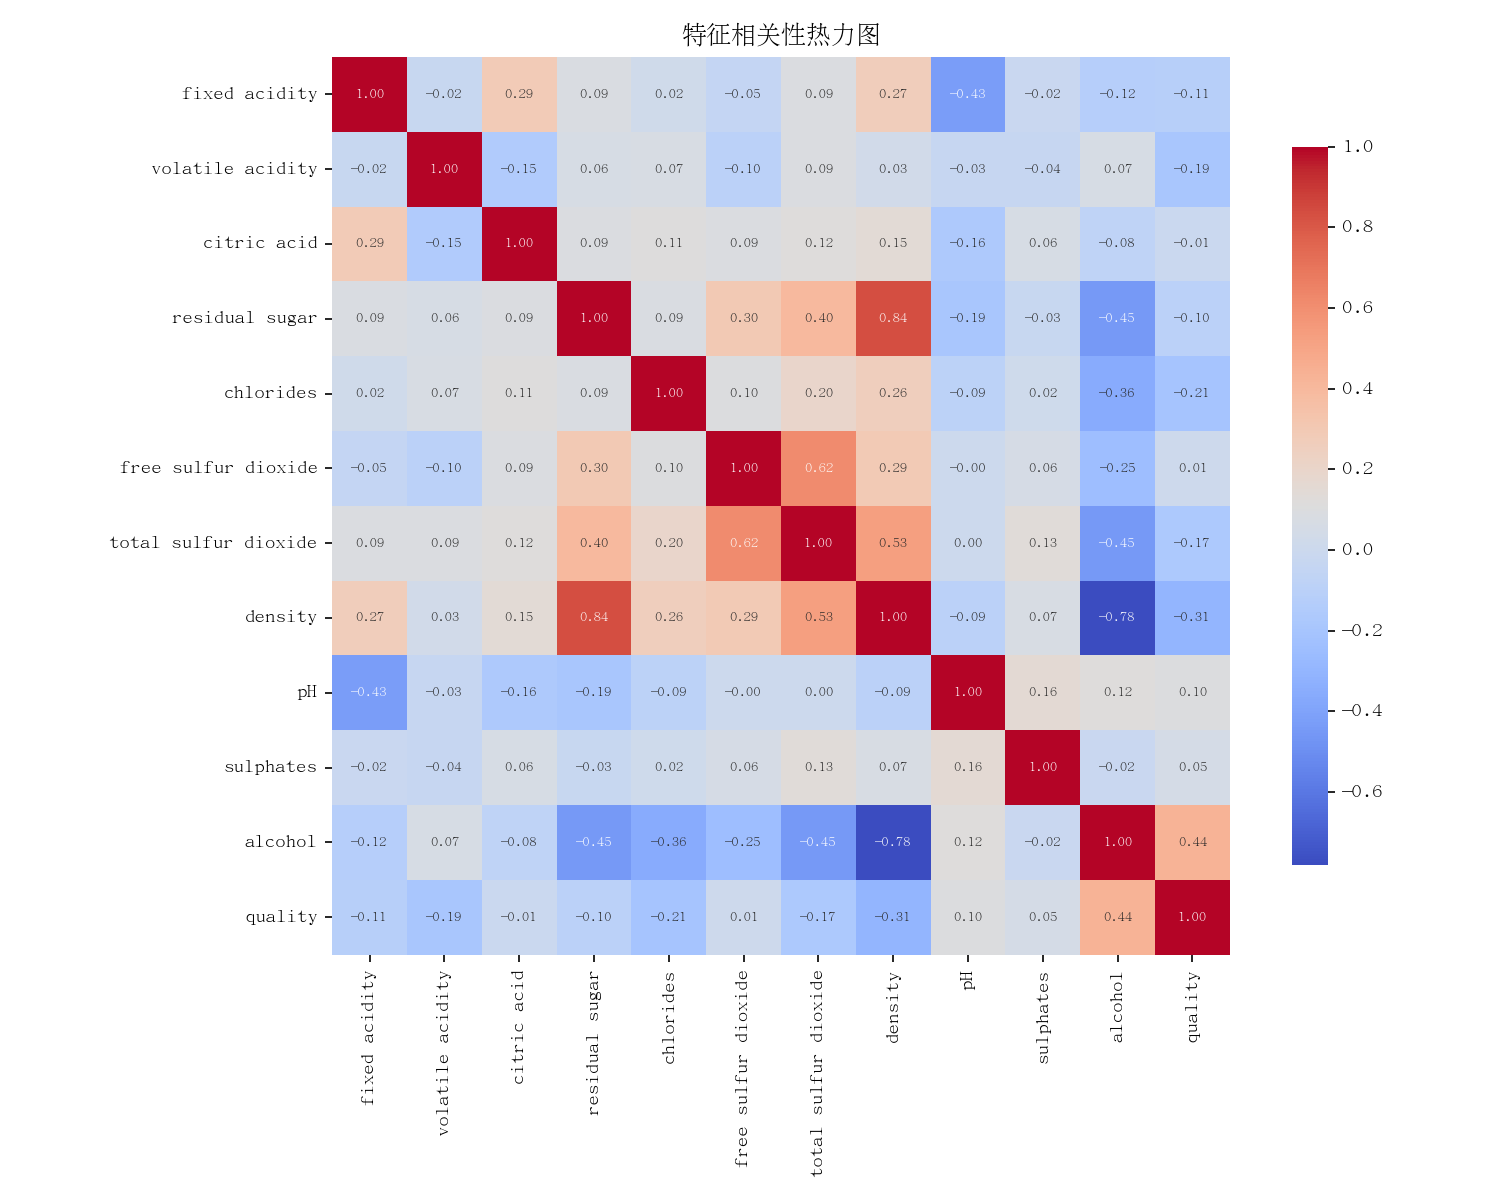
\includegraphics[width=0.78\textwidth]{eda_corr_heatmap.png}
  \caption{特征相关性热力图}
  \label{fig:eda_corr}
\end{figure}

\subsection{模型与结果}
对四种模型分别进行 5 折交叉验证网格搜索调参，并在测试集上评估。各模型的准确率、
精确率、召回率与宏平均 F1 见表~\ref{tab:ml}。模型对比与随机森林特征重要性分别见
图~\ref{fig:cmp} 与图~\ref{fig:imp}。

\begin{table}[H]
  \centering
  \caption{四种机器学习模型测试集性能对比}
  \label{tab:ml}
  \begin{tabular}{lcccc}
    \toprule
    模型 & 准确率 & 精确率 & 召回率 & 宏平均 F1 \\
    \midrule
    SVM        & 0.617 & 0.616 & 0.660 & 0.622 \\
    决策树     & 0.650 & 0.647 & 0.644 & 0.645 \\
    \textbf{随机森林} & \textbf{0.735} & \textbf{0.748} & \textbf{0.723} & \textbf{0.734} \\
    逻辑回归   & 0.522 & 0.524 & 0.567 & 0.520 \\
    \bottomrule
  \end{tabular}
\end{table}

\begin{figure}[H]
  \centering
  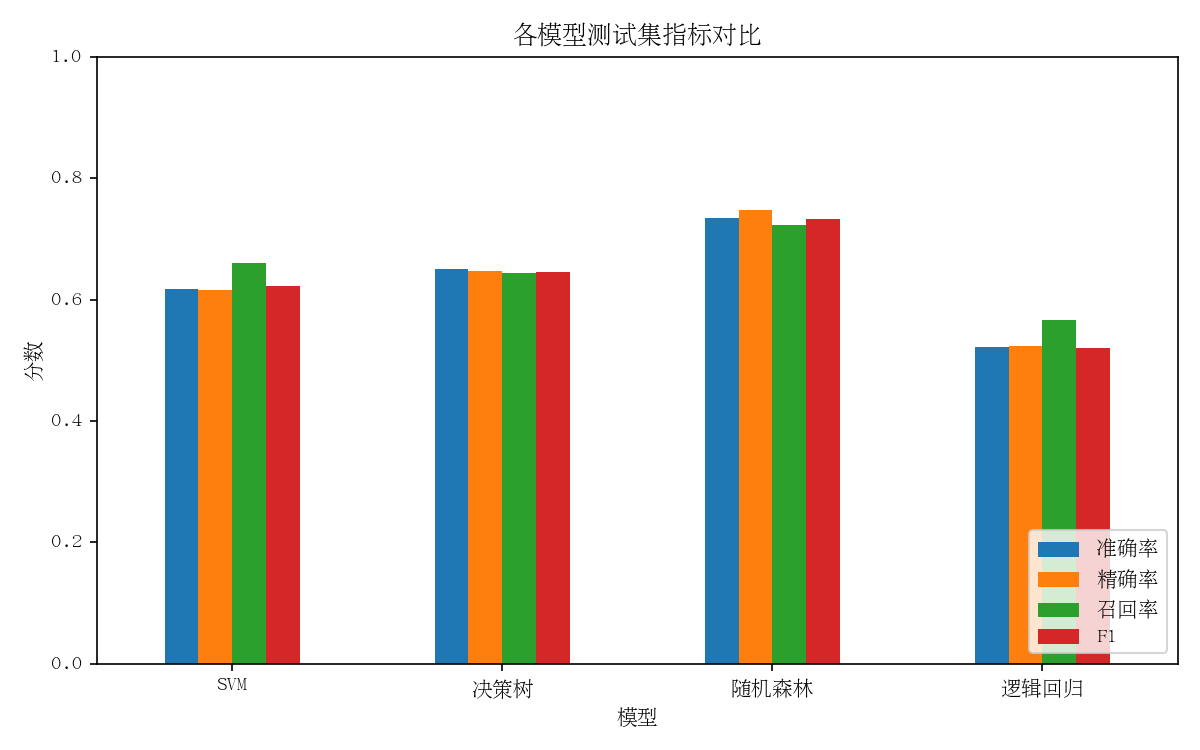
\includegraphics[width=0.8\textwidth]{model_compare.png}
  \caption{各模型测试集指标对比}
  \label{fig:cmp}
\end{figure}

\begin{figure}[H]
  \centering
  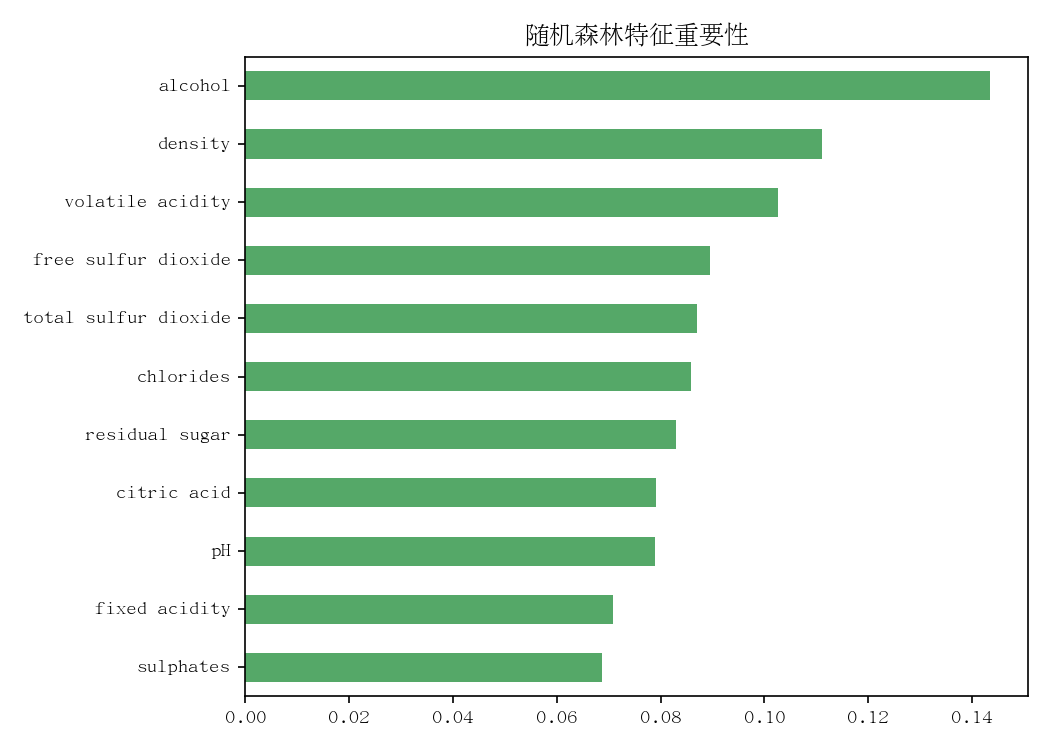
\includegraphics[width=0.7\textwidth]{rf_feature_importance.png}
  \caption{随机森林特征重要性}
  \label{fig:imp}
\end{figure}

随机森林在所有指标上均显著优于其他模型，宏平均 F1 达 0.734；逻辑回归作为线性模型表现最差，
说明该任务存在较强的非线性关系。特征重要性显示酒精度、密度等理化指标对质量判别贡献最大。

\section{项目二：手写 AlexNet 图像分类}

\subsection{网络结构}
本项目不调用任何预置 AlexNet，而是使用基础算子逐层手工搭建。网络输入为 $1\times224\times224$
的灰度图（Fashion-MNIST 经 Resize 至 224），结构如下：

\begin{itemize}
  \item \textbf{特征提取（5 个卷积块）：}
  Conv1($1\!\to\!96$, $11\times11$, 步长 4) + ReLU + LRN + 最大池化；
  Conv2($96\!\to\!256$, $5\times5$) + ReLU + LRN + 最大池化；
  Conv3($256\!\to\!384$, $3\times3$) + ReLU；
  Conv4($384\!\to\!384$, $3\times3$) + ReLU；
  Conv5($384\!\to\!256$, $3\times3$) + ReLU + 最大池化，输出 $256\times6\times6$。
  \item \textbf{分类器（3 个全连接）：}
  Dropout + 全连接($9216\!\to\!4096$) + ReLU；
  Dropout + 全连接($4096\!\to\!4096$) + ReLU；
  全连接($4096\!\to\!10$)。
\end{itemize}
模型参数量约 58.3M。

\subsection{训练与评估}
采用交叉熵损失与带动量的随机梯度下降（SGD，动量 0.9，权重衰减 $5\times10^{-4}$），
初始学习率 0.01，每 10 轮衰减为 1/10，共训练 15 轮，按验证集准确率保存最优模型。
训练过程中验证集最高准确率为 0.9232。训练曲线见图~\ref{fig:curves}。

\begin{figure}[H]
  \centering
  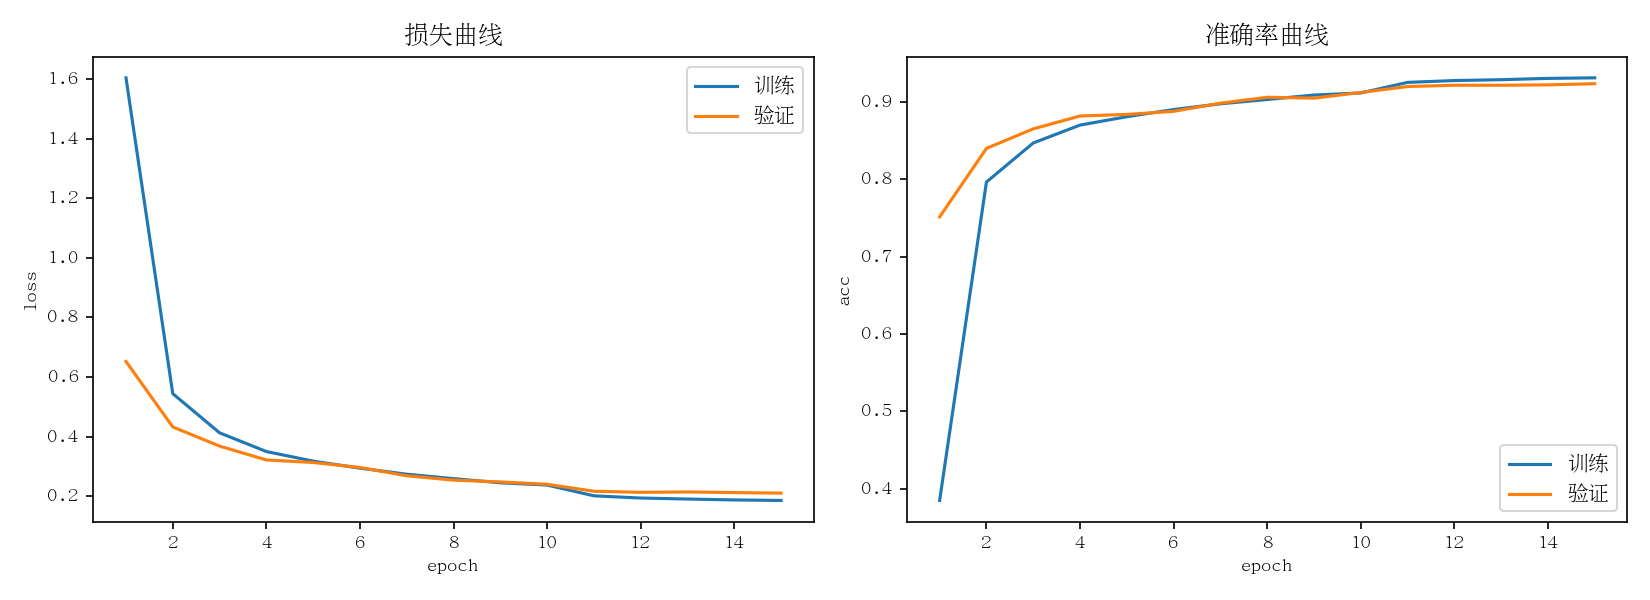
\includegraphics[width=0.95\textwidth]{curves.png}
  \caption{训练/验证 损失与准确率曲线}
  \label{fig:curves}
\end{figure}

在 10000 张测试图像上，模型最终准确率为 \textbf{91.55\%}，宏平均 F1 为 \textbf{0.915}。
混淆矩阵与预测样例分别见图~\ref{fig:cm} 与图~\ref{fig:samples}。其中“衬衫”类与“T恤”“套衫”
“外套”之间存在较多混淆，符合 Fashion-MNIST 上该类目视觉相似度高的普遍规律。

\begin{figure}[H]
  \centering
  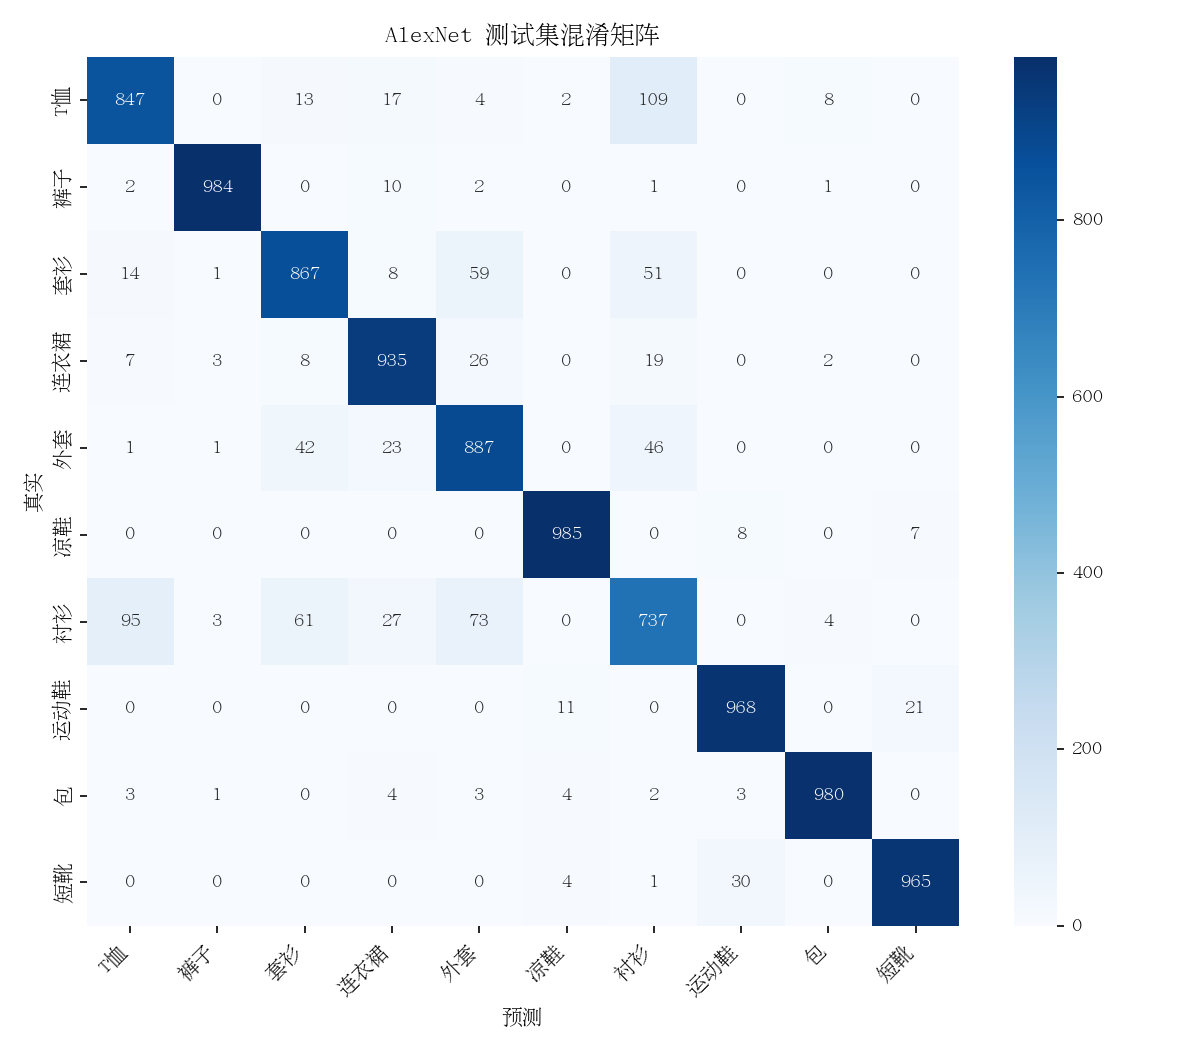
\includegraphics[width=0.85\textwidth]{confusion_matrix.png}
  \caption{AlexNet 测试集混淆矩阵}
  \label{fig:cm}
\end{figure}

\begin{figure}[H]
  \centering
  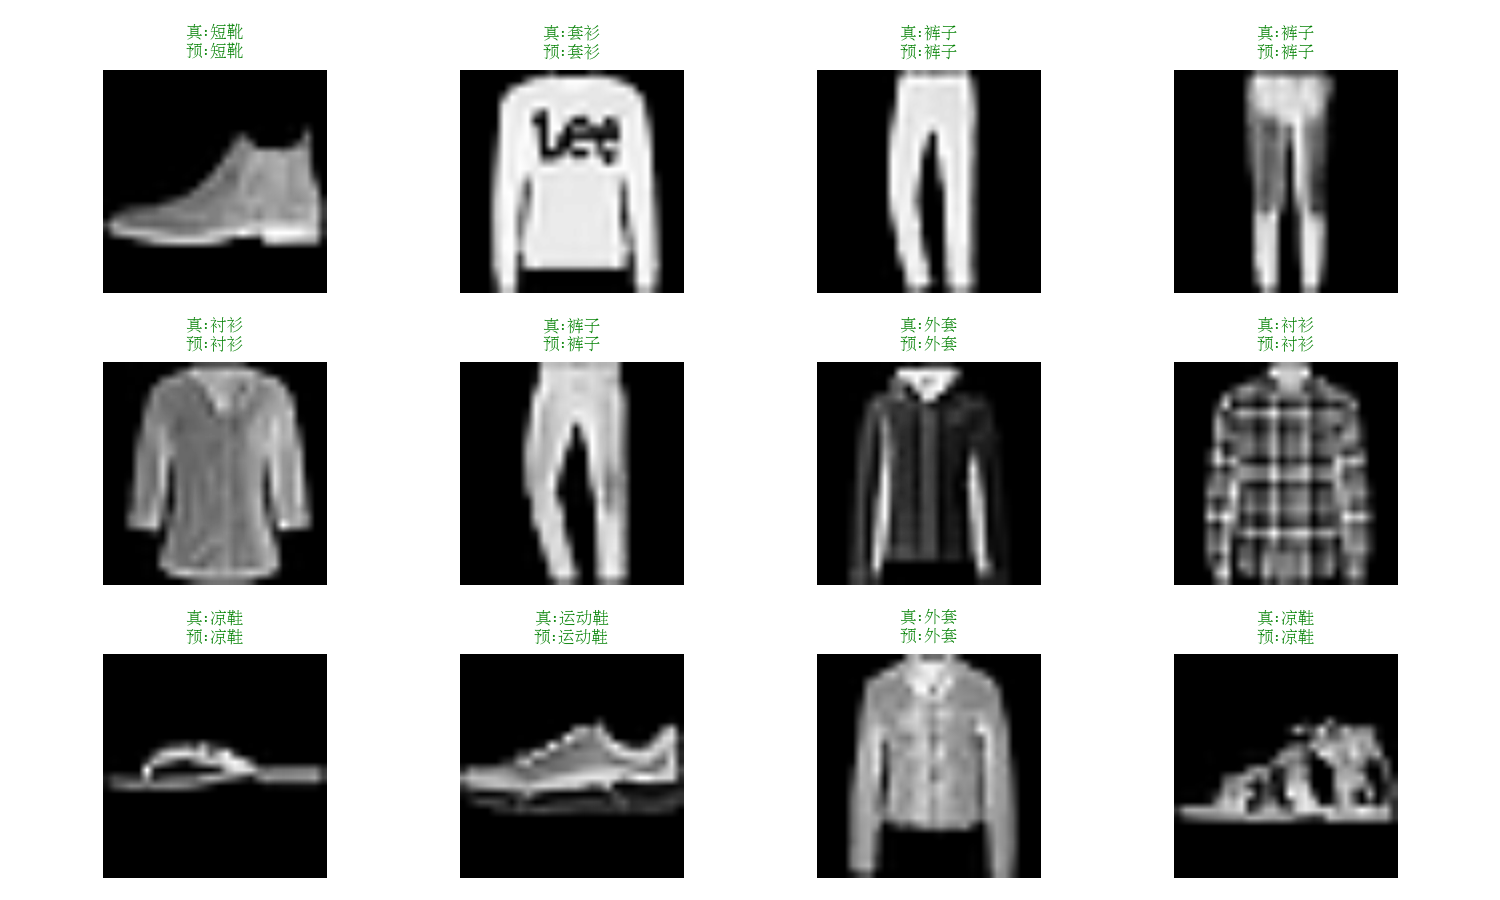
\includegraphics[width=0.85\textwidth]{samples.png}
  \caption{测试集预测样例（绿色为正确，红色为错误）}
  \label{fig:samples}
\end{figure}

\section{结论}
本报告完整实践了两类机器学习任务。项目一表明集成学习（随机森林）在结构化数据多分类上
优于单一模型与线性模型；项目二验证了手写 AlexNet 在图像分类上的有效性，测试准确率达 91.55\%。
后续可通过数据增强、批归一化、更深网络结构以及更充分的超参数搜索进一步提升性能。

\begin{thebibliography}{9}
\bibitem{alexnet} Krizhevsky A, Sutskever I, Hinton G E.
ImageNet Classification with Deep Convolutional Neural Networks.
\textit{Advances in Neural Information Processing Systems (NeurIPS)}, 2012.
\bibitem{wine} Cortez P, et al. Modeling wine preferences by data mining from
physicochemical properties. \textit{Decision Support Systems}, 2009, 47(4): 547--553.
\bibitem{sklearn} Pedregosa F, et al. Scikit-learn: Machine Learning in Python.
\textit{JMLR}, 2011, 12: 2825--2830.
\end{thebibliography}

\end{document}
